\sloppy
Python Variabel Type  \par
\noindent 
Satu dari fitur yang paling powerful dari sebuah bahasa pemrograman adalah kemampuan untuk memanipulasi $  $variabel. Sebuah variabel adalah nama yang merujuk ke sebuah nilai. \par
\vspace{12pt}
\noindent 
Pernyataan pemberian nilai $  $(assigment statement) akan memberikan nilai pada variabel: \par
\vspace{12pt}


 %%%%%%%%%%%%  Table No:1 Here %%%%%%%%%%%%%%


\begin{table}[H]
\centering
\begin{adjustbox}{width=\textwidth}
\begin{tabular}{ p{0.33in}p{7.3in} }
\hhline{--}
\multicolumn{1}{|p{0.33in}}{123} & \multicolumn{1}{|p{7.3in}|}{>>> pesan = "Apa kabar, bro ?">>> n = 17>>> pi = 3.14159} & \hline
\end{tabular}
\end{adjustbox}
\end{table}


 %%%%%%%%%%%%  Table No:1 Ends Here %%%%%%%%%%%%%%


\vspace{12pt}
\noindent 
Contoh diatas melakukan tiga pemberian nilai. Yang pertama memberikan nilai string $  $"Apa kabar, bro ?" $  $pada variabel bernama $  $pesan. Yang Kedua memberikan nilai integer $  $17 $  $kepada $  $n, dan yang ketiga memberikan nilai bilangan floating-point $  $3.14159 $  $kepada variabel dengan nama $  $pi. \par
\vspace{12pt}
\noindent 
Token pemberian nilai, tanda $  $=, agar tidak bingung jangan disamakan dengan tanda $  $sama dengan, yang mana menggunakan token $  $== $  $. Pernyataan pemberian nilai mengikat sebuah $  $nama $  $di sebelah kiri dari operator, dan nilainya, di sebelah kanannya. Inilah mengapa kamu akan mendapatkan error jika kamu menulis: \par
\vspace{12pt}


 %%%%%%%%%%%%  Table No:2 Here %%%%%%%%%%%%%%


\begin{table}[H]
\centering
\begin{adjustbox}{width=\textwidth}
\begin{tabular}{ p{0.33in}p{7.3in} }
\hhline{--}
\multicolumn{1}{|p{0.33in}}{123} & \multicolumn{1}{|p{7.3in}|}{>>> 17 = nFile "<interactive input>", line 1SyntaxError: can't assign to literal} & \hline
\end{tabular}
\end{adjustbox}
\end{table}


 %%%%%%%%%%%%  Table No:2 Ends Here %%%%%%%%%%%%%%


\vspace{12pt}
\noindent 
Ketika membaca atau menulis kode, katakan dalam hati "n diberikan nilai 17". Jangan katakan "n sama dengan 17". \par
\vspace{12pt}
\noindent 
Cara umum untuk merepresentasikan variabel pada kertas adalah dengan menulis namanya dengan tanda panah mengarah ke nilai variabelnya. Gambar jenis ini dinamakan $  $state snapshot $  $karena ia memperlihatkan state atau kondisi dari setiap variabel pada instan waktu tertentu. (Pikirkan ini sebagai variabel keadaan pikiran). Diagram ini memperlihatkan hasil dari pengeksekusian pernyataan pemberian nilai: \par
\vspace{12pt}
\vspace{12pt}
\noindent 


 %%%%%%%%%%%%  Figure/Image No:1 here %%%%%%%%%%%%%%


\begin{figure}[H]
\begin{center}
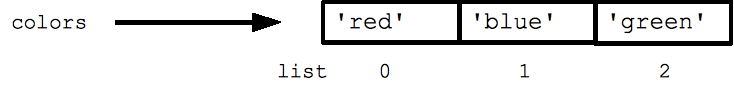
\includegraphics[width=4.16in,height=1.19in]{/home/ubuntu/Django/mysite/docx2latex/uploads_new_lazy_free/Variabel_Type_Python_DIR/media/image1.png}
\end{center}
\end{figure}


 %%%%%%%%%%%%  Figure/Image No:1 Ends Here %%%%%%%%%%%%%%


\vspace{12pt}
\vspace{12pt}
\noindent 
Jika kamu meminta interpreter untuk menilai sebuah variabel, ia akan menghasilkan nilai dari variabel terkait pada waktu sekarang: \par
\vspace{12pt}


 %%%%%%%%%%%%  Table No:3 Here %%%%%%%%%%%%%%


\begin{table}[H]
\centering
\begin{adjustbox}{width=\textwidth}
\begin{tabular}{ p{0.33in}p{7.3in} }
\hhline{--}
\multicolumn{1}{|p{0.33in}}{123456} & \multicolumn{1}{|p{7.3in}|}{>>> pesan'Apa kabar, bro ?'>>> n17>>> pi3.14159} & \hline
\end{tabular}
\end{adjustbox}
\end{table}


 %%%%%%%%%%%%  Table No:3 Ends Here %%%%%%%%%%%%%%


\vspace{12pt}
\noindent 
Kita menggunakan variabel-variabel pada program untuk "mengingat" hal-hal, misalnya skore terkini ketika sedang ada pertandingan sepak bola. Tapi variabel tetaplah $  $variabel. Ini artinya mereka bisa berganti seiring waktu, sama halnya dengan papan skor pada pertandingan bola. Kamu bisa memberikan nilai pada variabel, dan kemudian memberikan nilai lainnya pada variabel yang sama. (Ini berbeda dari sudut pandang matematika. Pada matematika, jika kamu memberi 'x' nilai 3, itu tidak bisa mengubah link nilai menjadi nilai yang berbeda pada pertengahan perhitungan yang kamu lakukan!) \par
\vspace{12pt}


 %%%%%%%%%%%%  Table No:4 Here %%%%%%%%%%%%%%


\begin{table}[H]
\centering
\begin{adjustbox}{width=\textwidth}
\begin{tabular}{ p{0.33in}p{7.3in} }
\hhline{--}
\multicolumn{1}{|p{0.33in}}{123456789} & \multicolumn{1}{|p{7.3in}|}{>>> hari = "Kamis">>> hari'Kamis'>>> hari = "Jumat">>> hari'Jumat'>>> hari = 21>>> hari21} & \hline
\end{tabular}
\end{adjustbox}
\end{table}


 %%%%%%%%%%%%  Table No:4 Ends Here %%%%%%%%%%%%%%


\vspace{12pt}
\noindent 
Kamu akan menyadari kita mengubah nilai dari $  $hari $  $sebanyak tiga kali, dan ketika pemberian nilai yang ketiga kita bahkan membuatnya merujuk pada nilai yang berbeda tipe dari yang sebelumnya. \par
\vspace{12pt}
\noindent 
Pemrograman itu kebanyakan tentang bagaimana komputer mengingat sesuatu, misal, $  $Jumlah panggilan tak terjawab pada handphone mu, $  $dan kemudian mengatur untuk memperbaharui atau merubah variabel ketika kamu melewatkan panggilan lainnya. \par
\vspace{12pt}
\noindent 
 Nama Variabel dan Keywords \par
\vspace{12pt}
\noindent 
Nama variabel $  $bisa ditulis panjang. Mereka bisa berisi huruf maupun digit angka, tapi harus diawali dengan huruf atau underscore. Meskipun dibolehkan untuk menggunakan huruf besar, tapi pada umumnya kita tidak menggunakannya. Jika kamu menggunakannya, ingat kalau besar kecilnya huruf itu berpengaruh. $  $Wayandan $  $wayan $  $itu merupakan dua variabel yang berbeda. \par
\vspace{12pt}
\noindent 
Karakter underscore (  $  \_  $ ) bisa ada pada nama. Biasanya digunakan pada nama yang terdiri dari lebih dari satu kata, misalnya seperti $  $nama $  \_  $saya $  $atau $  $harga $  \_  $jual $  \_  $produk. \par
\vspace{12pt}
\noindent 
Ada beberapa situasi yang mana nama yang diawali dengan underscore memiliki arti yang spesial, jadi aturan yang paling aman untuk pemula adalah memulai sebuah nama hanya dengan menggunakan huruf kecil. \par
\vspace{12pt}
\noindent 
Jika kamu memberikan variabel nama yang ilegal, kamu akan mendapatkan syntax error: \par
\noindent 
\href{https://tutorkeren.com/artikel/python-3-rle-bab-2-variabel-ekspresi-dan-pernyataan.htm}{?}
 \par


 %%%%%%%%%%%%  Table No:5 Here %%%%%%%%%%%%%%


\begin{table}[H]
\centering
\begin{adjustbox}{width=\textwidth}
\begin{tabular}{ p{0.33in}p{7.3in} }
\hhline{--}
\multicolumn{1}{|p{0.33in}}{123456} & \multicolumn{1}{|p{7.3in}|}{>>> 123doremi = "tiga not awal"SyntaxError: invalid syntax>>> gaji $  \$  $ = 1000000SyntaxError: invalid syntax>>> class = "Kewirausahaan 121"SyntaxError: invalide syntax} & \hline
\end{tabular}
\end{adjustbox}
\end{table}


 %%%%%%%%%%%%  Table No:5 Ends Here %%%%%%%%%%%%%%


\vspace{12pt}
\noindent 
123doremi $  $adalah ilegal karena tidak dimulai dengan huruf. $  $gaji $  \$  $ $  $juga ilegal karena memakai karakter ilegal, tanda dollar seharusnya tidak boleh. Tapi apa yang salah dengan $  $class $  $? \par
\vspace{12pt}
\noindent 
Ternyata karena $  $class $  $merupakan satu dari $  $keyword $  $(kata kunci) $  $yang dimiliki $  $Python. Keyword mendefinisikan aturan syntax bahasa dan struktur, dan maka dari itu tidak diperkenakan untuk digunakan sebagai nama variabel. \par
\vspace{12pt}
\noindent 
Python memiliki tiga puluhan keyword (dan hingga kini Python masih meningkatkannya dengan memperkenalkan atau menghilangkan satu atau dua): \par


 %%%%%%%%%%%%  Table No:6 Here %%%%%%%%%%%%%%


\begin{table}[H]
\centering
\begin{adjustbox}{width=\textwidth}
\begin{tabular}{ p{0.44in}p{0.32in}p{0.49in}p{0.57in}p{0.44in}p{0.57in} }
\hhline{~~~~~~}
\multicolumn{1}{p{0.44in}}{and} & \multicolumn{1}{p{0.32in}}{as} & \multicolumn{1}{p{0.49in}}{assert} & \multicolumn{1}{p{0.57in}}{break} & \multicolumn{1}{p{0.44in}}{class} & \multicolumn{1}{p{0.57in}}{continue} & \hhline{~~~~~~}
\multicolumn{1}{p{0.44in}}{def} & \multicolumn{1}{p{0.32in}}{del} & \multicolumn{1}{p{0.49in}}{elif} & \multicolumn{1}{p{0.57in}}{else} & \multicolumn{1}{p{0.44in}}{except} & \multicolumn{1}{p{0.57in}}{exec} & \hhline{~~~~~~}
\multicolumn{1}{p{0.44in}}{finally} & \multicolumn{1}{p{0.32in}}{for} & \multicolumn{1}{p{0.49in}}{from} & \multicolumn{1}{p{0.57in}}{global} & \multicolumn{1}{p{0.44in}}{if} & \multicolumn{1}{p{0.57in}}{import} & \hhline{~~~~~~}
\multicolumn{1}{p{0.44in}}{in} & \multicolumn{1}{p{0.32in}}{is} & \multicolumn{1}{p{0.49in}}{lambda} & \multicolumn{1}{p{0.57in}}{nonlocal} & \multicolumn{1}{p{0.44in}}{not} & \multicolumn{1}{p{0.57in}}{or} & \hhline{~~~~~~}
\multicolumn{1}{p{0.44in}}{pass} & \multicolumn{1}{p{0.32in}}{raise} & \multicolumn{1}{p{0.49in}}{return} & \multicolumn{1}{p{0.57in}}{try} & \multicolumn{1}{p{0.44in}}{while} & \multicolumn{1}{p{0.57in}}{with} & \hhline{~~~~~~}
\multicolumn{1}{p{0.44in}}{yield} & \multicolumn{1}{p{0.32in}}{True} & \multicolumn{1}{p{0.49in}}{False} & \multicolumn{1}{p{0.57in}}{None} & \multicolumn{1}{p{0.44in}}{} & \multicolumn{1}{p{0.57in}}{} & \hline
\end{tabular}
\end{adjustbox}
\end{table}


 %%%%%%%%%%%%  Table No:6 Ends Here %%%%%%%%%%%%%%


\vspace{12pt}
\noindent 
Kamu mungkin berniat untuk menyimpan daftar ini untuk mempermudah. Jika si interpreter komplain mengenai satu sari nama variabel mu dan kamu tidak tahu mengapa demikian, lihatlah apakah nama variabel yang kamu buat masuk daftar diatas. Jika iya, ganti dengan nama yang lain. \par
\vspace{12pt}
\noindent 
Programer umumnya memilih nama untuk variabel mereka agar memiliki arti dan bisa dimengerti oleh pembaca manusia -- dengan demikian maka akan membantu si programer untuk mendokumentasikan, atau mengingat, apa gunanya variabel tersebut. \par
\vspace{12pt}
\vspace{12pt}
\noindent 
Pemula biasanya bingung dengan maksud dari "berguna untuk pembaca manusia" dengan "berguna untuk mesin atau komputer". Jadi mungkin mereka akan berpikir salah, bahwa ketika mereka memanggil beberapa variabel dengan nama $  $averageatau $  $pi, itu akan dengain ajaib menghitung sebuah average / rata-rata, atau dengan ajaib tahu kalau pi memiliki nilai seperti 3.14159. Tidak ! Komputer tidak akan mengerti itu, komputer tidak akan mengerti apa yang kamu inginkan dari variabel hanya karena namanya unik. \par
\vspace{12pt}
\noindent 
Jadi kamu mungkin akan menemui beberapa instruktur yang memang sengaja tidak memilih nama yang berarti ketika mereka mengajar pemula -- bukan karena kita tidak menganggap itu merupakan kebiasaan yang baik, tapi karena kita mencoba untuk menekankan ulang pesannya kepada kalian -- seorang programer -- harus menulis sendiri kode program untuk menghitung average-nya, dan kamu harus menulis pernyataan pemberian nilai untuk memberikan nilai pada variabel $  $pidengan nilai yang kamu inginkan. \par
\vspace{12pt}
\noindent 
 Pernyataan \par
\vspace{12pt}
\noindent 
Sebuah $  $pernyataan $  $(statement) adalah perintah/instruksi yang bisa dieksekusi/dijalankan oleh Python interpreter. Hingga kini kita hanya baru melihat pernyataan pemberian nilai. Beberapa jenis lain dari pernyataan yang akan kita lihat dengan singkat adalah pernyataan $  $while, pernyataan $  $for, pernyataan $  $if, dan pernyataan $  $import. (Ada banyak lagi yang lainnya!) \par
\vspace{12pt}
\noindent 
Ketika kamu mengetikan pernyataan pada command line, Python akan menjalankannya. Pernyataannya sendiri tidak menghasilkan hasil apapun. \par
\vspace{12pt}
\noindent 
Variabel tidak lain hanyalah lokasi memori reserved untuk menyimpan nilai. $  $Ini berarti bahwa ketika Anda membuat variabel Anda memesan beberapa ruang di memori. \par
\vspace{12pt}
\noindent 
Berdasarkan tipe data sebuah variabel, penafsir mengalokasikan memori dan memutuskan apa yang dapat disimpan dalam memori yang dipesan. $  $Oleh karena itu, dengan menetapkan tipe data yang berbeda ke variabel, Anda dapat menyimpan bilangan bulat, desimal atau karakter dalam variabel ini. \par
\vspace{12pt}
\noindent 
Variabel adalah lokasi memori yang dicadangkan untuk menyimpan nilai-nilai. Ini berarti bahwa ketika Anda membuat sebuah variabel Anda memesan beberapa ruang di memori. Variabel menyimpan data yang dilakukan selama program dieksekusi, yang natinya isi dari variabel tersebut dapat diubah oleh operasi - operasi tertentu pada program yang menggunakan variabel.\vspace{\baselineskip}
\vspace{\baselineskip}
Variabel dapat menyimpan berbagai macam $  $\href{https://www.belajarpython.com/2015/05/tipe-data-python.html}{tipe data}
. Di dalam pemrograman Python, variabel mempunyai sifat yang dinamis, artinya variabel Python tidak perlu didekralasikan tipe data tertentu dan variabel Python dapat diubah saat program dijalankan. \par
\noindent 
\vspace{\baselineskip}
\vspace{\baselineskip}
Penulisan variabel Python sendiri juga memiliki aturan tertentu, yaitu : \par
\noindent 
\vspace{\baselineskip}
1. Karakter pertama harus berupa huruf atau garis bawah/underscore $  $ $  \_  $ \par
\noindent 
\vspace{\baselineskip}
2. Karakter selanjutnya dapat berupa huruf, garis bawah/underscore $  $ $  \_  $ $  $atau angka \par
\noindent 
\vspace{\baselineskip}
3. Karakter pada nama variabel bersifat sensitif (case-sensitif). Artinya huruf kecil dan huruf besar dibedakan. Sebagai contoh, variabel $  $namaDepan $  $dan $  $namadepan $  $adalah variabel yang berbeda.\vspace{\baselineskip}
\vspace{\baselineskip}
Untuk mulai membuat variabel di Python caranya sangat mudah, Anda cukup menuliskan variabel lalu mengisinya dengan suatu nilai dengan cara menambahkan tanda sama dengan $  $= $  $diikuti dengan nilai yang ingin dimasukan. \par
\vspace{12pt}
\noindent 
Menilai Ekspresi \par
\vspace{12pt}
\noindent 
Sebuah ekspresi merupakan perpaduan antara nilai, variabel, operator, dan pemanggilan fungsi. Jika kamu mengetik sebuah ekspresi pada Python prompt, maka si interpreter akan $  $menilainya $  $dan menampilkan hasilnya: \par
\vspace{12pt}


 %%%%%%%%%%%%  Table No:7 Here %%%%%%%%%%%%%%


\begin{table}[H]
\centering
\begin{adjustbox}{width=\textwidth}
\begin{tabular}{ p{0.33in}p{7.3in} }
\hhline{--}
\multicolumn{1}{|p{0.33in}}{1234} & \multicolumn{1}{|p{7.3in}|}{>>> 1 + 12>>> len("hello")5} & \hline
\end{tabular}
\end{adjustbox}
\end{table}


 %%%%%%%%%%%%  Table No:7 Ends Here %%%%%%%%%%%%%%


\vspace{12pt}
\noindent 
Pada contoh ini $  $len $  $merupakan fungsi built-in yang ada di Python yang akan menghasilkan jumlah karakter dari sebuah string. Sebelumnya kita sudah melihat fungsi $  $print $  $dan $  $type, jadi ini adalah contoh fungsi ketiga kita! \par
\vspace{12pt}
\noindent 
Proses $  $penilaian dari sebuah ekspresi $  $akan menghasilkan sebuah nilai, itulah mengapa ekspresi bisa ada di sisi sebelah kanan dari pernyataan pemberian nilai. $  $Nilai $  $dengan sendirinya $  $adalah ekspresi $  $sederhana, $  $dan begitu juga $  $variabel. \par
\vspace{12pt}


 %%%%%%%%%%%%  Table No:8 Here %%%%%%%%%%%%%%


\begin{table}[H]
\centering
\begin{adjustbox}{width=\textwidth}
\begin{tabular}{ p{0.33in}p{7.3in} }
\hhline{--}
\multicolumn{1}{|p{0.33in}}{12345678} & \multicolumn{1}{|p{7.3in}|}{>>> 1717>>> y = 3.14>>> x = len("hello")>>> x5>>> y3.14} & \hline
\end{tabular}
\end{adjustbox}
\end{table}


 %%%%%%%%%%%%  Table No:8 Ends Here %%%%%%%%%%%%%%


\vspace{12pt}
\noindent 
Menetapkan Nilai ke Variabel \par
\vspace{12pt}
\noindent 
Variabel Python tidak memerlukan deklarasi eksplisit untuk memesan ruang memori. $  $Deklarasi terjadi secara otomatis saat Anda menetapkan nilai ke variabel. $  $Tanda sama (=) digunakan untuk menetapkan nilai pada variabel. \par
\vspace{12pt}
\noindent 
Operand di sebelah kiri = operator adalah nama variabel dan operan di sebelah kanan = operator adalah nilai yang tersimpan dalam variabel. $  $Misalnya  \par
\vspace{12pt}
\noindent 
counter~=~100~~~~~~~    $  \#  $ An integer assignment \par
\noindent 
miles~~~=~1000.0~~~~    $  \#  $ A floating point \par
\noindent 
name~~~~=~"John"~~~~    $  \#  $ A string \par
\vspace{12pt}
\noindent 
print counter \par
\noindent 
print miles \par
\noindent 
print name \par
\vspace{12pt}
\noindent 
Di sini, 100, 1000.0 dan "John" adalah nilai yang diberikan untuk $  $melawan $  $, $  $mil $  $, dan $  $variabel $  $nama $  $masing-masing. $  $Ini menghasilkan hasil sebagai berikut  \par
\vspace{12pt}
\noindent 
100 \par
\noindent 
1000.0 \par
\noindent 
John \par
\vspace{12pt}
\noindent 
Beberapa Tugas \par
\noindent 
Python memungkinkan Anda untuk menetapkan nilai tunggal ke beberapa variabel secara bersamaan. $  $Misalnya  \par
\vspace{12pt}
\noindent 
a = b = c = 1 \par
\vspace{12pt}
\noindent 
Di sini, sebuah objek bilangan bulat dibuat dengan nilai 1, dan ketiga variabel ditugaskan ke lokasi memori yang sama. $  $Anda juga dapat menetapkan beberapa objek ke beberapa variabel. $  $Misalnya  \par
\vspace{12pt}
\noindent 
a,b,c = 1,2,"john" \par
\vspace{12pt}
\noindent 
Di sini, dua objek bilangan bulat dengan nilai 1 dan 2 masing-masing diberikan pada variabel a dan b masing-masing, dan satu objek string dengan nilai "john" diberikan ke variabel c. \par
\vspace{12pt}
\noindent 
Tipe data standar \par
\noindent 
Data yang tersimpan dalam memori bisa bermacam-macam. $  $Misalnya, usia seseorang disimpan sebagai nilai numerik dan alamatnya disimpan sebagai karakter alfanumerik. $  $Python memiliki berbagai jenis data standar yang digunakan untuk menentukan operasi yang mungkin dilakukan pada mereka dan metode penyimpanan untuk masing-masing metode. \par
\vspace{12pt}
\noindent 
Python memiliki lima tipe data standar - \par
\vspace{12pt}
\noindent 
Angka \par
\noindent 
Tali \par
\noindent 
Daftar \par
\noindent 
Tuple \par
\noindent 
Kamus \par
\noindent 
Nomor Python \par
\vspace{12pt}
\noindent 
Nomor tipe data menyimpan nilai numerik. $  $Nomor objek dibuat saat Anda memberikan nilai pada mereka. $  $Misalnya  \par
\vspace{12pt}
\noindent 
var1 = 1 \par
\noindent 
var2 = 10 \par
\vspace{12pt}
\noindent 
Anda juga dapat menghapus referensi ke objek nomor dengan menggunakan del statement. $  $Sintaks dari pernyataan del adalah - \par
\vspace{12pt}
\noindent 
del var1[,var2[,var3[....,varN]]]] \par
\vspace{12pt}
\noindent 
Anda dapat menghapus satu objek atau beberapa objek dengan menggunakan pernyataan del. $  $Misalnya  \par
\vspace{12pt}
\noindent 
del var \par
\noindent 
del var $  \_  $a, var $  \_  $b \par
\vspace{12pt}
\noindent 
Python mendukung empat jenis numerik yang berbeda  \par
\vspace{12pt}
\noindent 
int (bilangan bulat yang ditandatangani) \par
\vspace{12pt}
\noindent 
Panjang (bilangan bulat panjang, mereka juga bisa diwakili dalam oktal dan heksadesimal) \par
\vspace{12pt}
\noindent 
float (floating point real value) \par
\vspace{12pt}
\noindent 
kompleks (bilangan kompleks) \par
\vspace{12pt}
\noindent 
Python memungkinkan Anda untuk menggunakan huruf kecil l dengan panjang, tapi disarankan agar Anda hanya menggunakan huruf besar L untuk menghindari kebingungan dengan nomor 1.  \par
\noindent 
Python menampilkan bilangan bulat panjang dengan huruf besar L. \par
\vspace{12pt}
\noindent 
Sebuah bilangan kompleks terdiri dari sepasang bilangan floating-point yang diinisialisasi langsung yang dinotasikan dengan x + yj, di mana x dan y adalah bilangan real dan j adalah unit imajiner. \par
\vspace{12pt}
\noindent 
String Python \par
\vspace{12pt}
\noindent 
String dengan Python diidentifikasi sebagai kumpulan karakter bersebelahan yang ditunjukkan dalam tanda petik. $  $Python memungkinkan untuk kedua pasang tanda kutip tunggal atau ganda. $  $Subset string dapat diambil dengan menggunakan operator slice ([] dan [:]) dengan indeks mulai dari 0 pada awal string dan bekerja dengan cara mereka dari -1 di akhir. \par
\vspace{12pt}
\noindent 
Tanda plus (+) adalah operator concatenation string dan tanda bintang (*) adalah operator pengulangan. $  $Misalnya  \par
\vspace{12pt}
\vspace{12pt}
\noindent 
str = 'Hello World!' \par
\vspace{12pt}
\noindent 
print~str~~~~~~~~   $  \#  $ Prints complete string \par
\noindent 
print str[0]~~~~~~  $  \#  $ Prints first character of the string \par
\noindent 
print str[2:5]~~~~  $  \#  $ Prints characters starting from 3rd to 5th \par
\noindent 
print str[2:]~~~~~  $  \#  $ Prints string starting from 3rd character \par
\noindent 
print~str~*~2~~     $  \#  $ Prints string two times \par
\noindent 
print str + "TEST"  $  \#  $ Prints concatenated string \par
\vspace{12pt}
\noindent 
Ini akan menghasilkan hasil sebagai berikut - \par
\vspace{12pt}
\noindent 
Hello World! \par
\noindent 
H \par
\noindent 
llo \par
\noindent 
llo World! \par
\noindent 
Hello World!Hello World! \par
\noindent 
Hello World!TEST \par
\vspace{12pt}
\noindent 
Daftar Python \par
\vspace{12pt}
\noindent 
Daftar adalah jenis data majemuk Python yang paling serbaguna. $  $Daftar berisi item yang dipisahkan dengan tanda koma dan dilampirkan dalam tanda kurung siku ([]). $  $Sampai batas tertentu, daftar serupa dengan array di C. Salah satu perbedaan di antara keduanya adalah bahwa semua item yang termasuk dalam daftar dapat terdiri dari tipe data yang berbeda. \par
\vspace{12pt}
\noindent 
Nilai yang tersimpan dalam daftar dapat diakses menggunakan operator slice ([] dan [:]) dengan indeks mulai dari 0 di awal daftar dan bekerja dengan cara mereka untuk mengakhiri -1. $  $Tanda plus (+) adalah daftar operator concatenation, dan asterisk (*) adalah operator pengulangan. $  $Misalnya  \par
\vspace{12pt}
\noindent 
 $  \#  $!/usr/bin/python \par
\vspace{12pt}
\noindent 
list = [ 'abcd', 786 , 2.23, 'john', 70.2 ] \par
\noindent 
tinylist = [123, 'john'] \par
\vspace{12pt}
\noindent 
print~list~~~~~~~~   $  \#  $ Prints complete list \par
\noindent 
print list[0]~~~~~~  $  \#  $ Prints first element of the list \par
\noindent 
print list[1:3]~~~~  $  \#  $ Prints elements starting from 2nd till 3rd  \par
\noindent 
print list[2:]~~~~~  $  \#  $ Prints elements starting from 3rd element \par
\noindent 
print tinylist * 2~  $  \#  $ Prints list two times \par
\noindent 
print list + tinylist  $  \#  $ Prints concatenated lists \par
\vspace{12pt}
\noindent 
Ini menghasilkan hasil sebagai berikut - \par
\vspace{12pt}
\noindent 
['abcd', 786, 2.23, 'john', 70.200000000000003] \par
\noindent 
abcd \par
\noindent 
[786, 2.23] \par
\noindent 
[2.23, 'john', 70.200000000000003] \par
\noindent 
[123, 'john', 123, 'john'] \par
\noindent 
['abcd', 786, 2.23, 'john', 70.200000000000003, 123, 'john'] \par
\vspace{12pt}
\noindent 
Tupel Python \par
\vspace{12pt}
\noindent 
Sebuah tupel adalah jenis data urutan lain yang serupa dengan daftar. $  $Sebuah tupel terdiri dari sejumlah nilai yang dipisahkan dengan koma. $  $Tidak seperti daftar, bagaimanapun, tupel tertutup dalam tanda kurung. \par
\vspace{12pt}
\noindent 
Perbedaan utama antara daftar dan tupel adalah: Daftar tertutup dalam tanda kurung ([]) dan elemen dan ukurannya dapat diubah, sementara tupel dilampirkan dalam tanda kurung (()) dan tidak dapat diperbarui. $  $Tupel bisa dianggap sebagai $  $daftar $  $hanya-baca $  $. $  $Misalnya - \par
\vspace{12pt}
\noindent 
 $  \#  $!/usr/bin/python \par
\vspace{12pt}
\noindent 
tuple = ( 'abcd',~786 , 2.23, 'john', 70.2  ) \par
\noindent 
tinytuple = (123, 'john') \par
\vspace{12pt}
\noindent 
print~tuple~~~~~~~~~   $  \#  $ Prints complete list \par
\noindent 
print tuple[0]~~~~~~~  $  \#  $ Prints first element of the list \par
\noindent 
print tuple[1:3]~~~~~  $  \#  $ Prints elements starting from 2nd till 3rd  \par
\noindent 
print tuple[2:]~~~~~~  $  \#  $ Prints elements starting from 3rd element \par
\noindent 
print~tinytuple~* 2    $  \#  $ Prints list two times \par
\noindent 
print tuple + tinytuple  $  \#  $ Prints concatenated lists \par
\noindent 
Ini menghasilkan hasil sebagai berikut - \par
\noindent 
('abcd', 786, 2.23, 'john', 70.200000000000003) \par
\noindent 
abcd \par
\noindent 
(786, 2.23) \par
\noindent 
(2.23, 'john', 70.200000000000003) \par
\noindent 
(123, 'john', 123, 'john') \par
\noindent 
('abcd', 786, 2.23, 'john', 70.200000000000003, 123, 'john') \par
\vspace{12pt}
\noindent 
Kode berikut tidak valid dengan tupel, karena kami mencoba memperbarui tupel, yang tidak diizinkan. $  $Kasus serupa dimungkinkan dengan daftar - \par
\vspace{12pt}
\noindent 
tuple = ( 'abcd',~786 , 2.23, 'john', 70.2  ) \par
\noindent 
list = [ 'abcd', 786 ,~2.23, 'john', 70.2  ] \par
\noindent 
tuple[2]~=~1000~    $  \#  $ Invalid syntax with tuple \par
\noindent 
list[2]~=~1000~~    $  \#  $ Valid syntax with list \par
\vspace{12pt}
\noindent 
Kamus Python \par
\vspace{12pt}
\noindent 
Kamus Python adalah jenis tipe tabel hash. $  $Mereka bekerja seperti array asosiatif atau hash yang ditemukan di Perl dan terdiri dari pasangan kunci-nilai. $  $Kunci kamus bisa hampir sama dengan tipe Python, tapi biasanya angka atau string. $  $Nilai, di sisi lain, bisa menjadi objek Python yang sewenang-wenang. \par
\vspace{12pt}
\noindent 
Kamus ditutupi oleh kurung kurawal ( $  \{  $ $  \}  $) dan nilai dapat diberikan dan diakses menggunakan kawat gigi persegi ([]). $  $Misalnya - \par
\vspace{12pt}
\noindent 
 $  \#  $!/usr/bin/python \par
\vspace{12pt}
\noindent 
dict =  $  \{  $ $  \}  $ \par
\noindent 
dict['one'] = "This is one" \par
\noindent 
dict[2]~~~~ = "This is two" \par
\vspace{12pt}
\noindent 
tinydict =  $  \{  $'name': 'john','code':6734, 'dept': 'sales' $  \}  $ \par
\vspace{12pt}
\vspace{12pt}
\noindent 
print dict['one']~~ ~~~  $  \#  $ Prints value for 'one' key \par
\noindent 
print dict[2]~~~~~~~~~~  $  \#  $ Prints value for 2 key \par
\noindent 
print~tinydict~~~~~~~~   $  \#  $ Prints complete dictionary \par
\noindent 
print tinydict.keys()~~  $  \#  $ Prints all the keys \par
\noindent 
print tinydict.values()  $  \#  $ Prints all the values \par
\noindent 
Ini menghasilkan hasil sebagai berikut - \par
\noindent 
This is one \par
\noindent 
This is two \par
\noindent 
 $  \{  $'dept': 'sales', 'code': 6734, 'name': 'john' $  \}  $ \par
\noindent 
['dept', 'code', 'name'] \par
\noindent 
['sales', 6734, 'john'] \par
\vspace{12pt}
\noindent 
Kamus tidak memiliki konsep keteraturan antar elemen. $  $Tidak benar mengatakan bahwa unsur-unsurnya "rusak"; $  $Mereka hanya unordered. \par
\vspace{12pt}
\noindent 
Konversi Tipe Data \par
\vspace{12pt}
\noindent 
Terkadang, Anda mungkin perlu melakukan konversi antara jenis built-in. $  $Untuk mengonversi antar jenis, Anda cukup menggunakan nama jenis sebagai fungsi. \par
\noindent 
Ada beberapa fungsi built-in untuk melakukan konversi dari satu tipe data ke tipe data yang lain. $  $Fungsi ini mengembalikan objek baru yang mewakili nilai yang dikonversi. \par
\vspace{12pt}
\noindent 
Pembagian nilai $  $a $  $dan $  $b $  $menghasilkan $  $3 $  $(integer). Mengapa demikian? \par
\vspace{12pt}
\noindent 
Karena nilai $  $a $  $dan $  $b $  $bertipe integer, maka hasilnya pun berupa integer. \par
\vspace{12pt}
\noindent 
Bagaimana agar hasilnya ada komanya? \par
\vspace{12pt}
\noindent 
Tentu kita harus merubah tipe variabel $  $a $  $dan $  $b $  $menjadi bilangan pecahan (float) dulu, baru setelah itu dibagi. \par
\vspace{12pt}
\noindent 
a = 10 \par
\noindent 
b = 3 \par
\noindent 
c = float(a) / float(b)  $  \#  $output: 3.3333333333333335 \par
\vspace{12pt}
\noindent 
print c \par
\vspace{12pt}
\noindent 
Fungsi $  $float() $  $akan mengubah nilai $  $a $  $menjadi $  $10.0 $  $dan $  $b $  $menjadi $  $3.0. \par
\vspace{12pt}
\noindent 
Fungsi-fungsi untuk mengubah tipe data: \par
\vspace{12pt}
\noindent 
int() $  $untuk mengubah menjadi integer; \par
\vspace{12pt}
\noindent 
long() $  $untuk mengubah menjadi integer panjang; \par
\vspace{12pt}
\noindent 
float() $  $untuk mengubah menjadi float; \par
\vspace{12pt}
\noindent 
bool() $  $untuk mengubah menjadi boolean; \par
\vspace{12pt}
\noindent 
chr() $  $untuk mengubah menjadi karakter; \par
\vspace{12pt}
\noindent 
str() $  $untuk mengubah menjadi string. \par
\vspace{12pt}
\noindent 
bin() $  $untuk mengubah menjadi bilangan Biner. \par
\vspace{12pt}
\noindent 
hex() $  $untuk mengubah menjadi bilangan Heksadesimal. \par
\vspace{12pt}
\noindent 
oct() $  $untuk mengubah menjadi bilangan okta. \par
\vspace{12pt}
\vspace{12pt}

